\documentclass[../distribution_theory_notes.tex]{subfiles}
\begin{document}
\section{Aula 07 - 13 de Setembro, 2024}
\subsection{Motivações}
\begin{itemize}
	\item O Espaço das Funções Teste.
\end{itemize}
\subsection{O Espaço das Funções Teste}
Tendo toda essa teoria geral sobre TVS's, focaremos na apresentação do espaço \(\mathcal{D}'(\Omega )\) das distribuições em \(\Omega \) como o dual topológico do TVS \(\mathcal{C}_{c}^{\infty}(\Omega ).\) O primeiro passo é dotar \(\mathcal{C}_{c}^{\infty}(\Omega )\) da topologia limite indutivo da sequência \(\{\mathcal{C}_{c}^{\infty}(K_{j})\}_{j\in \mathbb{N}}\) de espaços de Fréchet, onde \(\{K_{j}\}_{j}\) é um esgotamento arbitrário de \(\Omega \), a base topológica que sustenta o \(\mathcal{D}'(\Omega )\), fazendo dele esse espaço gigantesco que é, tanto na generalidade de seus elementos quanto na facilidade de convergir dentro dele.

Feito isso, caracterizamos os elementos de \(\mathcal{D}'(\Omega )\) por meio de estimativas, tal como fizemos com \(\mathcal{E}'(\Omega )\) e \(\mathcal{S}'\), e descreveremos a tal da convergência super simples dele. Vale destacar que \(\mathcal{C}_{c}^{\infty}(\Omega )\hookrightarrow \mathcal{C}^{\infty}(\mathbb{R}^{n})\) e, quando \(\Omega =\mathbb{R}^{n}\), tem-se também
\[
	\mathcal{C}_{c}^{\infty}(\mathbb{R}^{n})\hookrightarrow \mathcal{S}(\mathbb{R}^{n})\hookrightarrow \mathcal{C}^{\infty}(\mathbb{R}^{n}) \Rightarrow \mathcal{E}'(\mathbb{R}^{n})\hookrightarrow \mathcal{S}'(\mathbb{R}^{n})\hookrightarrow \mathcal{D}'(\mathbb{R}^{n}).
\]
Se tudo der certo, daremos alguns exemplos de distribuições e faremos um pequeno comentário sobre a convolução de funções, indispensável para o desenvolvimento da Análise de Fourier.

\begin{def*}
	Se \(\Omega \) é um aberto de \(\mathbb{R}^{n}\), o \textbf{espaço de funções teste} é o conjunto
	\[
		\mathcal{C}_{c}^{\infty}(\Omega )\coloneqq \{\varphi \in \mathcal{C}^{\infty}(\mathbb{R}^{n}):\; \mathrm{supp}(\varphi )\text{ é compacto},\; \mathrm{supp}(\varphi )\subseteq \Omega \},
	\]
	ou seja, o conjunto de funções cujo suporte é um compacto contido em \(\Omega \). \(\square\)
\end{def*}

A topologia que adotaremos em \(\mathcal{C}_{c}^{\infty}(\Omega )\) é a topologia do limite indutivo dos \(\mathcal{C}_{c}^{\infty}(K_{j})\), tendo em vista que, se \(\{K_{j}\}_{j}\) é um esgotamento de \(\Omega \), fica claro que
\[
	\mathcal{C}_{c}^{\infty}(\Omega )=\bigcup_{j=1}^{\infty}\mathcal{C}_{c}^{\infty}(K_{j}),
\]
além de
\[
	\mathcal{C}_{c}^{\infty}(K_{j})\hookrightarrow \mathcal{C}_{c}^{\infty}(K_{j+1})
\]
ser uma inclusão de forma contínua. Observe que a topologia induzida não depende do esgotamento escolhido para \(\Omega \)!
\begin{tcolorbox}[
		skin=enhanced,
		title=Observação,
		fonttitle=\bfseries,
		colframe=black,
		colbacktitle=cyan!75!white,
		colback=cyan!15,
		colbacklower=black,
		coltitle=black,
		drop fuzzy shadow,
		%drop large lifted shadow
	]
	Se f e g são duas funções em \(\mathcal{C}_{c}^{\infty}(K)\), a combinação linear delas \(f+\lambda g\) também pertence ao mesmo conjunto para qualquer que seja o \(\lambda \) complexo, pois
	\[
		\mathrm{supp}(\lambda f)\subseteq \mathrm{supp}(f)\quad\&\quad \mathrm{supp}(f+g)\subseteq \mathrm{supp}(f)\cup \mathrm{supp}(g);
	\]
	de fato, esta última relação faz sentido pois
	\[
		f(x)+g(x)\neq 0 \Rightarrow f(x)\neq 0 \text{ ou }g(x)\neq 0,
	\]
	resultando em x sendo um elemento do suporte de uma delas, ou seja,
	\[
		x\in \mathrm{supp}(f)\cup \mathrm{supp}(g)\Rightarrow \mathrm{supp}(f+g)\subseteq \overline{\mathrm{supp}(f)\cup \mathrm{supp}(g)}=\mathrm{supp}(f)\cup \mathrm{supp}(g).
	\]
\end{tcolorbox}

Tendo um espaço e uma topologia, voltamos nossa atenção à descrição da convergência nesse espaço. Faremos isto por meio do
\begin{theorem*}
	Sejam \(\{\varphi_{j}\}_{j}\) e \(\varphi \) elementos de \(\mathcal{C}_{c}^{\infty}(\Omega )\). São equivalentes:
	\begin{itemize}
		\item[i)] Na topologia de \(\mathcal{C}_{c}^{\infty}(\Omega ),\; \varphi_{j}\rightarrow \varphi \) ;
		\item[ii)] Existe um compacto K contido em \(\Omega \) tal que K contém em si os suportes tanto de \(\varphi_{j}\) quanto de \(\varphi \) e \(\varphi_{j}\rightarrow \varphi \) em \(\mathcal{C}_{c}^{\infty}(K)\), isto é, para todo \(\alpha \) em \(\mathbb{Z}_{+}^{n}\),
		      \[
			      \sup_{x\in K}|\partial^{\alpha }\varphi_{j}(x)-\partial^{\alpha }\varphi (x)|\rightarrow 0.
		      \]
	\end{itemize}
\end{theorem*}
\begin{proof*}
	O fato de (ii) implicar (i) segue simplesmente  do Teorema do Limite indutivo, pois
	\[
		\mathcal{C}_{c}^{\infty}(K_{j})\hookrightarrow \mathcal{C}_{c}^{\infty}(\Omega ),
	\]
	donde segue que a convergência no ``menor'' resulta na convergência no ``Maior''. Do mesmo modo, escolhendo j tal que \(K\) esteja contido em \(K_{j}\), tem-se
	\[
		\mathcal{C}_{c}^{\infty}(K)\hookrightarrow \mathcal{C}_{c}^{\infty}(K_{j}),
	\]
	completando esta parte.

	Por outro lado, para ver como (i) resulta em (ii), sabemos que, em qualquer TVS,
	\[
		\varphi_{j}\rightarrow \varphi  \Longleftrightarrow \varphi_{j}-\varphi \rightarrow 0,
	\]
	então podemos admitir, sem perda de generalidade, que
	\[
		\varphi_{j}\substack{\mathcal{C}_{c}^{\infty}(\Omega ) \\ \longrightarrow \\ }0.
	\]
	Além disso, suponhamos que a segunda condição em (ii) seja falsa, permitindo que façamos a seguinte construção:

	Existe \(j_1\) em \(\mathbb{N}\) tal que \(\mathrm{supp}(\varphi_{j_1})\not\subseteq K_1\), donde concluímos que existe \(x_1\) em \(\Omega \) satisfazendo
	\[
		\varphi_{j_1}(x_1)\neq 0 \quad\&\quad x_1\not\in K_1,
	\]
	permitindo que suponhamos \(x_1\in K_2\) (caso contrário, basta substituir \(K_2\) pelo \(K_{\ell_1}\) com \(x\in K_{\ell_1}\)). Consequentemente, deve existir \(j_2\) maior que \(j_1\) satisfazendo, por sua vez,
	\[
		\mathrm{supp}(\varphi_{j_2})\not\subseteq K_2,
	\]
	já que, se não fosse o caso, existiria um compacto contendo o suporte de todas as \(\varphi_{j}\) para \(j\geq j_1\), contradizendo a nossa hipótese. Logo, como acima, podemos admitir que existe \(x_2\) em \(K_3\setminus{K_1}\) que torna verdadeira a relação \(\varphi_{j_2}(x_2)\neq 0\).

	Continuando o processo de maneira análoga, encontramos uma subsequência \(\{\varphi_{j_1}\}_{r\in \mathbb{N}}\) de \(\{\varphi_{j}\}_{j}\) e uma sequência \(\{x_1\}_{r}\) de pontos de \(\Omega \) tais que:
	\begin{align*}
		 & x_1\in K_{r+1}\setminus{K_r},\; \forall r; \text{ e} \\
		 & \varphi_{j_r}(x_r)\neq 0,\; \forall r.
	\end{align*}
	\begin{figure}[H]
		\begin{center}
			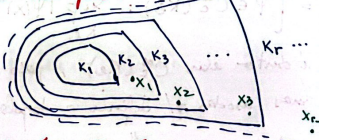
\includegraphics[height=0.5\textheight, width=0.5\textwidth, keepaspectratio]{./Images/points_construction_06.png}
		\end{center}
		\caption{construção dos pontos de \(\Omega \) e subsequência de \({\varphi_{j}}\).}
	\end{figure}

	Note que \(\{x_r\}_r\) não possui ponto de acumulação em \(\Omega \), pois, segundo a construção feita, as subsequências de \(\{x_r\}_r\) vão todas ou pro infinito, ou acumulam na fronteira de \(\Omega \):
	\[
		x_r\rightarrow a\in \Omega,\quad a\in K_r \subseteq \mathrm{int}(K_{r+1})\subseteq K_r.
	\]
	Com isso, \(x_{\ell }\) pertenceria a \(K_r\) para todo \(\ell \), que iria contradizer sua escolha.

	Nessas condições, pondo \(\delta_r = |\varphi_{j_r}(x_r)|>0\), vemos que
	\[
		W\coloneqq \{\varphi\in \mathcal{C}_{c}^{\infty}(\Omega ):\; |\varphi(x_r)|<\delta_r,\; r\in \mathbb{N}\}
	\]
	é convexo, equilibrado e com \(W\cap \mathcal{C}_{c}^{\infty}(K_{\ell})\) sendo um aberto de \(\mathcal{C}_{c}^{\infty}(K_{\ell})\) para todo \(\ell \) natural, fazendo-o um aberto de \(\mathcal{C}_{c}^{\infty}(\Omega )\) conforme o \hyperlink{inductive_limit}{\textit{teorema do limite indutivo}}.

	Com efeito, para ver que ele é convexo e equilibrado, basta notar que, se \(|\lambda |\leq 1\),
	\[
		|\lambda \varphi (x_r)| = |\lambda |\cdot |\varphi(x_r)|<\delta_r,
	\]
	e, se \(t\in [0,1]\) e \(\varphi , \psi\) são elementos de W, o mesmo vale para
	\[
		|(1-t)\varphi (x_r)+t\psi (x_r)|<(1-t)\delta_r+ t\delta_r = \delta_r,
	\]
	mostrando que \((1-t)\varphi + t\psi \in W\). Para provar que \(W\cap \mathcal{C}_{c}^{\infty}(K_{\ell})\) é aberto em \(\mathcal{C}_{c}^{\infty}(K_{\ell})\), observamos que apenas \(x_1,\dotsc ,x_{\ell -1}\) pertencem a \(K_{\ell}\) pela construção feita, tal que, se \(\psi_{0}\in W\cap \mathcal{C}_{c}^{\infty}(K_{\ell})\), então o conjunto
	\begin{align*}
		B & =\{\psi \in \mathcal{C}_{c}^{\infty}(K_{\ell}):\; \sup_{K_{\ell}}|\psi (x)-\psi_{0}(x)|<\delta_1-|\varphi_{0}(x_1)|\}\cap \dotsc \cap                                                         \\
		  & \cap \{\psi \in \mathcal{C}_{c}^{\infty}(K_{\ell}):\; \sup_{K_{\ell}}|\psi (x)-\psi_{0}(x)|<\delta_{\ell -1}-|\varphi_{0}(x_{\ell -1})|\}                                                     \\
		  & = \{\psi  \in \mathcal{C}_{c}^{\infty}(K_{\ell}):\; \sup_{K_{\ell}}|\psi (x)-\psi_{0}(x)|<\delta \},\quad \delta\coloneqq \min\limits_{i=1,2,\dotsc ,\ell -1}\{\delta_{i}-|\psi_{0}(x_{i})|\}
	\end{align*}
	é aberto em \(\mathcal{C}_{c}^{\infty}(K_{\ell})\) porque
	\[
		p_{\ell}(\psi )=\sup_{K_{\ell}}|\varphi(x)|
	\]
	é uma das seminormas usadas para definir a topologia de \(\mathcal{C}_{c}^{\infty}(K_{\ell})\), contendo \(\psi_{0}\) e contido em W: para \(i=1,2,\dotsc , \ell -1\)
	\[
		\psi\in B \Rightarrow |\psi(x_{i})|\leq |\psi (x_{i})-\psi_{0}(x_{i})|+|\psi_{0}(x_{i})| < (\delta_{i}-|\psi_{0}(x_{i})|)+|\psi_{0}(x_{i})| = \delta_{i}
	\]
	e \(\psi (x_{i})=0\) se i for maior ou igual a \(\ell .\)

	No entanto, a existência desse aberto impede que
	\[
		\varphi_{j}\substack{\mathcal{C}_{c}^{\infty}(\Omega ) \\ \longrightarrow \\ }0,
	\]
	tendo em vista que W contém a origem de \(\mathcal{C}_{c}^{\infty}(\Omega )\), mas não contém nenhuma das \(\varphi_{j_r}\), já que \(|\varphi_{j_r}(x_{r})|=\delta_r\) para cada r natural.

	Em conclusão, encontramos um compacto K de \(\Omega \) com \(\mathrm{supp}(\varphi_{j})\) contido nele para todo j natural, e isto completa a prova, pois se \(\varphi_{j}\rightarrow 0\) em \(\mathcal{C}_{c}^{\infty}(\Omega )\) e existe um natural \(\ell \) tal que \(\mathrm{supp}(\varphi_{j})\subseteq K_{\ell}\) para todo j natural, então dado \(m\in \mathbb{N}\), o conjunto
	\[
		\Omega_{\delta }=\{\psi \in \mathcal{C}_{c}^{\infty}(\Omega ):\; \sum\limits_{|\alpha |\leq m}^{}\sup_{K_{\ell}}|\partial^{\alpha }\psi (x)|<\delta \}
	\]
	é aberto em \(\mathcal{C}_{c}^{\infty}(\Omega )\) para todo \(\delta \) positivo. Portanto, para j suficientemente grande, \(\varphi_{j}\in \Omega_d\), o que nos dá
	\[
		\sup_{K_{\ell}}| \partial ^{\alpha }\varphi_{j}(x)|\substack{ \\ \longrightarrow \\ j\to \infty}0, \quad \forall \alpha \in \mathbb{Z}_{+}^{n},
	\]
	finalizando a prova. \qedsymbol
\end{proof*}
\begin{tcolorbox}[
		skin=enhanced,
		title=Observação,
		fonttitle=\bfseries,
		colframe=black,
		colbacktitle=cyan!75!white,
		colback=cyan!15,
		colbacklower=black,
		coltitle=black,
		drop fuzzy shadow,
		%drop large lifted shadow
	]
	Se \(K\subseteq \mathbb{R}^{n}\) é um compacto, então a topologia de \(\mathcal{C}_{c}^{\infty}(K)\) é dada pela seminormas
	\[
		p_{m}(\varphi )\coloneqq \sum\limits_{|\alpha |\leq m}^{}\sup_{K} |\partial^{\alpha }\varphi (x)|,
	\]
	pois se \(\{K_{j}\}_{j}\) esgota \(\mathbb{R}^{n},\) podemos supor que \(K_1\supseteq K\), possivelmente descartando os primeiros que não o contenham e começando com o primeiro que contenha K. Assim, para \(m, j\in \mathbb{N}\) e \(\varphi \in \mathcal{C}_{c}^{\infty}(K)\),
	\[
		p_{(m, j)}(\varphi )=p_{m}(\varphi),
	\]
	mostrando que
	\[
		p_{(m, j)}^{-1}((-\delta, \delta ))\cap \mathcal{C}_{c}^{\infty}(K)=p_{m}^{-1}((-\delta , \delta )).
	\]
\end{tcolorbox}
\begin{tcolorbox}[
		skin=enhanced,
		title=Observação,
		fonttitle=\bfseries,
		colframe=black,
		colbacktitle=cyan!75!white,
		colback=cyan!15,
		colbacklower=black,
		coltitle=black,
		drop fuzzy shadow,
		%drop large lifted shadow
	]
	As seminormas \(p_{(m, j)}\) de \(\mathcal{C}^{\infty}(\Omega )\) são contínuas em \(\mathcal{C}_{c}^{\infty}(\Omega )\). Com efeito, dados \(\psi_{0}\in \mathcal{C}_{c}^{\infty}(\Omega )\) e \(\delta \) positivo, temos
	\[
		V_{\delta }(\psi_{0})=\{\psi \in \mathcal{C}_{c}^{\infty}(\Omega ):\; p_{(m, j)}(\psi -\psi_{0})<\delta \}=V_{\delta }(0)+\psi_{0},
	\]
	onde \(V_{\delta }(0)\) é convexo, equilibrado e satisfaz
	\[
		V_{\delta }(0)\cap \mathcal{C}_{c}^{\infty}(K)=\{\psi \in \mathcal{C}_{c}^{\infty}(K):\; p_{(m, j)}(\psi )<\delta \}=\{\psi \in \mathcal{C}_{c}^{\infty}(K):\; p_{m}(\psi )<\delta \}
	\]
	pela observação anterior, onde K é um compacto de \(\Omega \) com \(\mathrm{int}(K)\neq\emptyset\) qualquer.
\end{tcolorbox}

\begin{theorem*}
	O espaço \(\mathcal{C}_{c}^{\infty}(\Omega )\) é sequencialmente completo.
\end{theorem*}
\begin{proof*}
	Com efeito, se \(\{\varphi_{j}\}_{j}\) é uma sequência de Cauchy, fica como exercício mostrar que existe K compacto de \(\Omega \) contendo o suporte de todas as \(\varphi_{j}\).

	Pela segunda observação feita, para todo m natural,
	\[
		p_{m}(\varphi_{j}-\varphi )\substack{ \\ \longrightarrow \\ j, r\to \infty}0,
	\]
	o que significa que \(\{\varphi_{j}\}_{j}\) é Cauchy em \(\mathcal{C}_{c}^{\infty}(K)\), o qual é completo. Portanto,
	\[
		\varphi_{j}\substack{\mathcal{C}_{c}^{\infty}(K)\\ \longrightarrow \\ j\to \infty}\varphi. \quad \text{qedsymbol}
	\]
\end{proof*}
O próximo teorema justifica a necessidade de considerar \(\mathcal{C}_{c}^{\infty}\) com outra topologia:
\begin{theorem*}
	O espaço \(\mathcal{C}_{c}^{\infty}(\Omega )\) não é completo com a topologia de \(\mathcal{C}^{\infty}(\Omega )\).
\end{theorem*}
\begin{proof*}
	Considerando o caso \(\Omega = \mathbb{R}\), uma \(\varphi \) em \(\mathcal{C}_{c}^{\infty}(\mathbb{R})\) com \(\mathrm{supp}(\varphi )\subseteq [-1, 1]\) e \( \varphi >0\) em \((-1, 1)\), definimos
	\[
		\varphi_{n}=\varphi (x+2)+\frac{1}{2}\varphi (x+4)+\frac{1}{3}\varphi (x+6)+\dotsc +\frac{1}{n}\varphi (x+2n),\quad x\in \mathbb{R},
	\]
	tal que \(\varphi_{n}\in \mathcal{C}_{c}^{\infty},\) a sequência \(\{\varphi_{n}\}\) é Cauchy em \(\mathcal{C}^{\infty}(\mathbb{R})\), mas
	\[
		\mathrm{supp}(\varphi )=[0, \infty),\quad \varphi = \lim_{n\to \infty}\varphi_{n},
	\]
	que não é um compacto. \qedsymbol
\end{proof*}

\end{document}
